\documentclass[journal,12pt,twocolumn]{IEEEtran}
\usepackage{graphicx}
\graphicspath{{./figs/}}{}
\usepackage{amsmath,amssymb,amsfonts,amsthm}
\newcommand{\myvec}[1]{\ensuremath{\begin{pmatrix}#1\end{pmatrix}}}
\providecommand{\norm}[1]{\lVert#1\rVert}
\usepackage{listings}
\usepackage{watermark}
\usepackage{titlesec}
\usepackage{caption}
\usepackage{enumitem}
\usepackage{extarrows}
\let\vec\mathbf
\lstset{
frame=single, 
breaklines=true,
columns=fullflexible
}
\thiswatermark{\centering \put(0,-105.0){
\includegraphics[scale=0.15]{/sdcard/IITH/vectors/12.10.2.11/figs/logo.png}} }
\title{\mytitle}
\title{
Assignment - 12.10.2.11
}
\author{Surajit Sarkar}
\begin{document}
\maketitle
\tableofcontents
\bigskip
\section{\textbf{Problem}}
Show that the vectors $2\hat{i}+3\hat{j}+4\hat{k}$ and $-4\hat{i}+6\hat{j}-8\hat{k}$ are collinear .
\section{\textbf{Solution}}
given
\begin{align}
\vec{a}=2\hat{i}+3\hat{j}+4\hat{k}\\
\vec{b}=4\hat{i}+6\hat{j}-8\hat{k}
\end{align}
\begin{align}
    \myvec{\vec{A}^{\top}\\ \vec{B}^{\top}}=1\\
\myvec{\vec{A}^{\top}\\ \vec{B}^{\top}}=\myvec{2&-3&4\\-4&6&-8}\\
\text{Forming the collinearity matrix}\\
\myvec{2&-3&4\\-4&6&-8} \xleftrightarrow{\frac{1}{2}R_1\to R_1}\myvec{1&-\frac{3}{2}&2\\-4&6&-8}\\
\xleftrightarrow{-\frac{1}{4}R_2\to R_2}\myvec{1&-\frac{3}{2}&2\\1&\frac{3}{2}&2}\\
\xleftrightarrow{R_2-1R_1\to R_2}\myvec{1&-\frac{3}{2}&2\\0&0&0}
\end{align}
  They have opposite direction \\
  \\
  Since $\vec{a}$ and $\vec{b}$ are same line they are collinear
\begin{lstlisting}
https://github.com/sssurajit/fwc/blob/main/vectors/12.10.2.11/codes/vector.py
\end{lstlisting}
Execute the code by using the command\\
\\
\textbf{python3 vector.py}\\
\section{\textbf{Figure}}
\begin{figure}[!ht]
    \centering
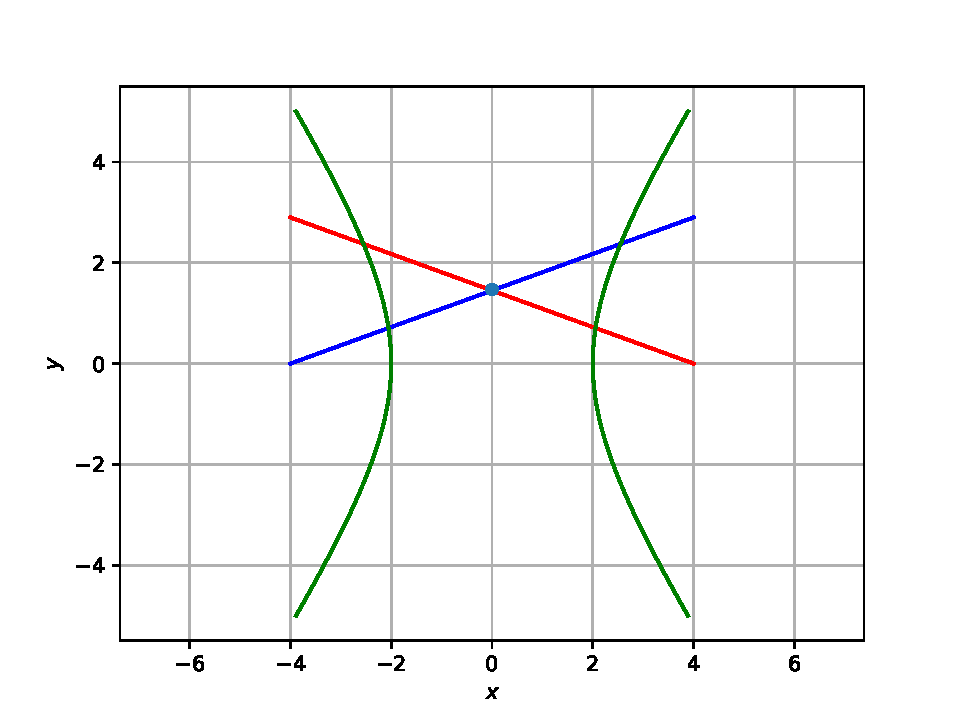
\includegraphics[width=\columnwidth]{/sdcard/IITH/vectors/12.10.2.11/figs/fig.pdf}
\caption{}
\label{fig:vec}
\end{figure}
\end{document}
